\section{Experimental Evaluation}\label{sec:results}

\subsection{Experimental Setup}
\label{sec:expSetup}

All GPU kernels that are used to evaluate S-L1 were executed on an NVIDIA GeForce GTX 680 GPU connected to 2GB of GPU memory with a total of 1,536 computing cores, each running at 1020MHz.
As described in Section~\ref{GPUBackground}, the GTX 680 is from the Kepler family and has 8 multiprocessors each with 192 computing cores,  and 64KB of on-chip memory (of which 48KB is assigned to shared memory).

Because the L1 cache of GTX 680 is disabled for application data by the vendor, we ran our experiments that examine the effects of a hardware L1 cache on a different GPU, namely an NVIDIA GTX 560 GPU with 336 computing cores connected to 1GB of GPU memory. 
The GTX 560 is a Fermi GPU containing 7 multiprocessors, each with 48 computing cores and
64kB of on-chip memory. 
The size of L1 cache can be configured to be 16KB or 48KB on this GPU;
we set it to 48KB (i.e., its maximum) for our experiments.

All GPU-based applications were implemented in CUDA, using CUDA toolkit and GPU driver release 6.0.37 installed on a 64-bit Ubuntu 12.04 Linux with kernel 3.5.0-23. 
All applications are compiled with the corresponding version of the {\it nvcc} compiler using optimization level three.

We applied S-L1 to the ten streaming applications listed in Table~\ref{tab:apps}. 
For each experiment, we ran the target application using different thread configurations,
and only considered the configuration with the best execution time for reporting and comparison purposes.
Specifically, we tested each application using 512 different thread configurations,
starting with 4 blocks of 128 threads (for a total of 512 threads) and increased the number of threads in 128 increments, up to 256 blocks of 1024 threads (for a total of 256K threads).

\begin{table*}[ht]
{
\begin{center}
%{\tiny
\resizebox{17cm}{2.1cm}
{
  \begin{tabular}{|p{2.8cm}|p{14.4cm}|p{3.5cm}|} \hline
         {\bf Application} & {\bf Description} &  {\bf Used number of data structures}\\
\hline
	  {Upper} &   {Converts all text in an input document from lowercase to uppercase.} &  {2}\\  \hline
	  {WC} &   {Counts the number of words and lines in an input document.} &  {1}\\ \hline
	  {DNA Assembly} & {merges fragments of a DNA sequence to reconstruct a larger sequence~\cite{dnaassembly}.} & {3}\\ \hline
	  {Opinion Finder} & {analyzes the sentiments of tweets associated with a given subject (i.e. a set of given keywords)~\cite{wilson2005opinionfinder}} &  {4}\\ \hline
	  {Inverted Index} & {Builds reverse index from a series of HTML files.} & {3}\\ \hline
	  {Page View Count} & {Counts the number of hits of each URL in a web log.} & {3}\\ \hline
          {MasterCard Affinity} & {finds all merchants that are frequently visited by customers of a target merchant X~\cite{}} & {3}\\ \hline
	  {Matrix Multiply} & {Calculates the multiplication of two input matrices. This is a naive version and does not use shared memory.} & {3}\\ \hline
	  {Grep} & {Finds the string matching a given pattern and outputs the line containing that string.} & {2 (1 in shared memory)}\\ \hline
	  {Kmeans} & {Partitions $n$ particles into $k$ clusters so that particles are assigned to the cluster with the nearest mean.} & {2 (1 in shared memory)}\\ \hline
  \end{tabular}
}
%}
\end{center}
}
\vspace{-0.0cm}
\caption{Our benchmark streaming applications, their description, and the number of data structures they use in their main loop.} %title of the table
\label{tab:apps}
\vspace{-0.0cm}
\end{table*}

\subsection{S-L1 performance evaluation}

\begin{figure}[t]
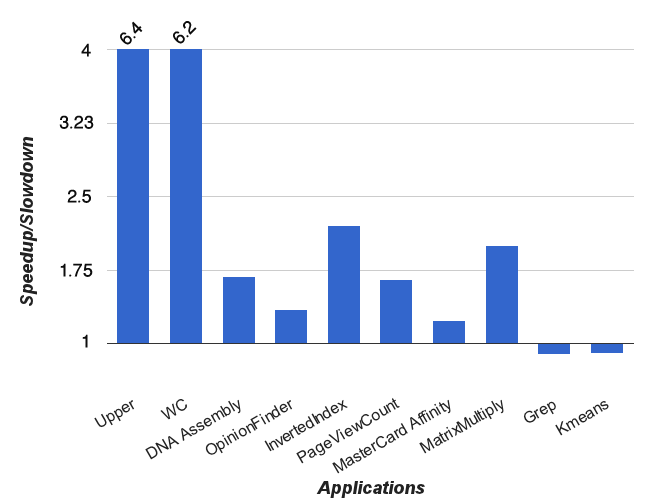
\includegraphics[scale=0.32]{1speedups.png}
\caption{Overall performance benefit of S-L1.}
\label{fig:perfbenefit}
\end{figure}

\begin{figure}[t]
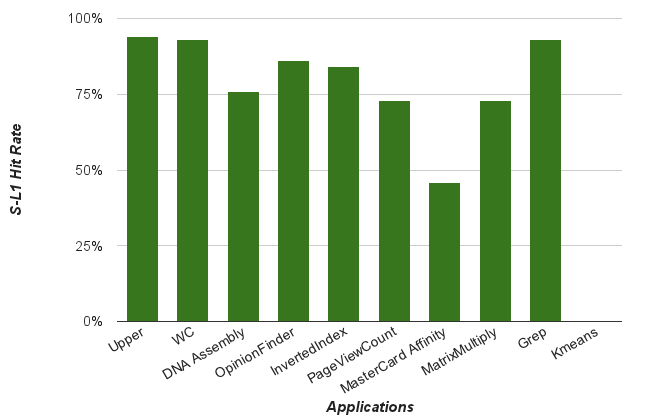
\includegraphics[scale=0.24]{3memoryAcceessReuction.png}
\caption{S-L1 hit rate.}
\label{fig:sl1hitrate}
\end{figure}




Figure~\ref{fig:perfbenefit} shows the performance of our 10 benchmark streaming applications when run with S-L1 relative to the performance of the same applications run without S-L1.
On average, these applications run 180\% faster than their non-caching counterparts. 
Some (e.g., \texttt{upper} and \texttt{wc}) run multiple times faster, while others (e.g., \texttt{grep} and \texttt{Kmeans}) experience slight slowdowns.

The benefits obtained from S-L1 depends on a number of factors.
First, the attained cache hit rate obviously has a large effect.
Figure~\ref{fig:sl1hitrate} depicts the S-L1 hit rate for all benchmarks. 
%%%%%%%
% MSt: 
% the following statement is simply not true in all cases, 
% which is why I commented it out 
% This hit rate translates into the percentage of the memory accesses that 
% otherwise had to leave the multiprocessors to be accessed -- either from L2 or DRAM. 
Overall, the hit rate is quite high, in part because most of the applications have high spatial
locality (which is to be expected for streaming applications). 
As an extreme example, consider \texttt{wc}, where each thread accesses a sequence of adjacent characters, so each S-L1 miss is typically followed by 15 hits, given a 16 byte cache line.
Kmeans is an exception: because the application allocates much of the shared memory for its own purposes, there is insufficient space for S-L1 cache lines, and hence the effective S-L1 hit rate is zero for this application.\footnote{
	Because Kmeans allocates space in shared memory dynamically at run time,
	the compiler cannot know that there is not enough space for S-L1 ---
	otherwise it potentially could have avoided adding the code required for S-L1.}

A second factor is the memory intensity of the applications; i.e., the ratio of memory access instructions to the total number of instructions executed.
Some applications (e.g., \texttt{upper} and \texttt{wc}) are memory bound and hence benefit from S-L1.
At the other extreme, \texttt{grep} performs worse despite having a high cache hit rate,
because it is compute intensive with its recursive algorithm and because it has a large number of branches with significant thread divergence.
The benefits of the caching layer is negated by the extra instructions that need to be executed because of the software implementation of S-L1.


\begin{figure}[t]
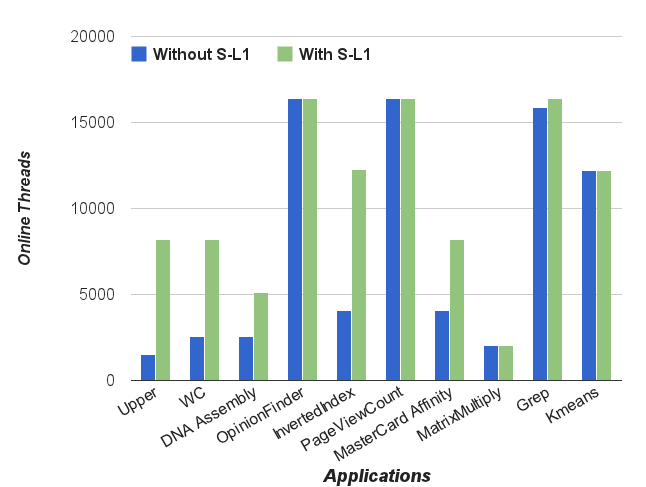
\includegraphics[scale=0.27]{8higherParallelism.png}
\caption{The level of parallelism with and without S-L1.}
\label{fig:levelprallelism}
\end{figure}

\begin{figure}[t]
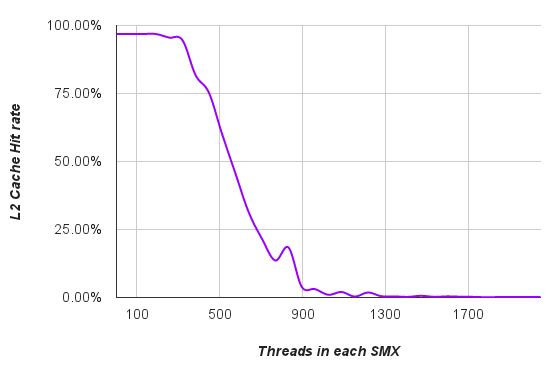
\includegraphics[scale=0.24]{10L2HitRateWC.png}
\caption{L2 hit rate for WC application.}
\label{fig:l2hitrate}
\end{figure}

A third factor is the degree to which S-L1 enables extra parallelism, thus improving the utilization of the GPU cores.
Figure~\ref{fig:levelprallelism} shows the optimal level of parallelism for each application with and without S-L1. 
(Note that only online threads are considered; i.e., threads that run at the same time on all multiprocessors, the maximum of which can be 16K threads on our GPU.)
With S-L1, applications can run with more threads without having to worry about thrashing the S-L1.
Without S-L1, applications typically need to limit the degree of parallelism to prevent L2 cache thrashing .
For example, Figure~\ref{fig:l2hitrate} shows the L2 cache hit rate of \texttt{wc} as a function of
the number of threads per SMX, where the cache hit rate drops to less than 1\% at 1,024 threads.







\subsection{Combining BigKernel and S-L1}

\begin{figure}[t]
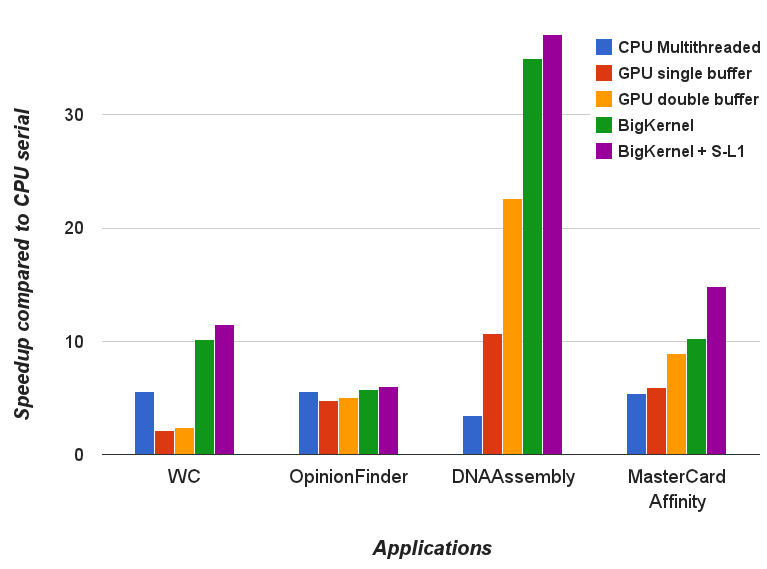
\includegraphics[scale=0.30]{11bigkernelAndSl1.png}
\caption{Performance speedup of various implementations over CPU serial version.}
\label{fig:bigkernelandsl1}
\end{figure}

For big data-style applications, the data will not fit in GPU memory because of the limited memory size. 
Hence, in this subsection, we consider the performance of four applications with data sets large enough to not fit in GPU memory.
We ran these applications under five different scenarios: 
\begin{enumerate}
\item CPU multithreaded when run on a 3.8GHz Intel Xeon Quad Core E5 connected to 16GB of quad-channel memory clocked at 1.8 GHz;
\item GPU using a single buffer to transfer data between CPU and GPU;
\item GPU using state-of-the-art double buffering to transfer data between CPU and GPU;
\item GPU using BigKernel; and
\item GPU using BigKernel combined with S-L1.
\end{enumerate}
Figure~\ref{fig:bigkernelandsl1} shows the results.
For all four applications, using BigKernel combined with S-L1 performs the best,
and for all but one application the performance is an order of magnitude better than the multithreaded CPU version.
On average, BigKernel combined with S-L1 performs 9\% faster than BigKernel alone.

The primary reason preventing BigKernel from performing better when combined with S-L1, we believe, is that adding S-L1 to BigKernel increases register pressure, often leading to register spillage, in part because BigKernel itself already uses many registers.

%\todo{Note, I don't buy your second reason, and I don't think you have evidence to back it up, so I cut  it.}
% First, since the memory accesses of BigKernel implementations are already
% coalesced, they often exhibit reasonable performance, leaving a rather small room for 
% improvement by S-L1.


\subsection{Comparing with hardware L1}
An interesting question is how our benchmarks would perform if a hardware L1 were available.
To answer this question, we executed our benchmark applications on an older GPU, the NVIDIA GTX 560,
that supports the L1 caching of application data (in contrast to the GTX~680).
Figure~\ref{fig:l1hitrate} shows the performance obtained with the L1 relative to running the
applications with L1 disabled. Overall, the performance gains with the L1 are limited to under 25\%
and in some cases result in minor slowdowns. We would expect that the performance with a hardware
L1 cache for application data on the GTX~680 would be far worse, because it has many more cores (192
vs.\ 48) but the same L1 cache size, which would result in increase L1 cache thrashing.

%\todo{Note: I cut out the Inverted Index cache hit rate graph and its description --- I don't think we need it...}

There are two further interesting observations.
First, unlike with S-L1, the hardware L1 cache increases the performance of \texttt{grep} reasonably well. 
We attribute this to the fact that the hardware L1 incurs no extra instruction overhead, which for \texttt{grep} is significant because it is already computationally intensive. 

Secondly, \texttt{wc},  \texttt{PageViewCount}, and \texttt{MasterCard Affinity} exhibit slowdown when L1 is enabled. 
We attribute this to the added memory transfers due to L1's large 128 byte cache lines (which is 4 times larger than L2's cache line size).
This phenomenon was originally observed by by Jia et al.~\cite{jia2012characterizing}.


\subsection{S-L1 overheads}

\begin{figure}[t]
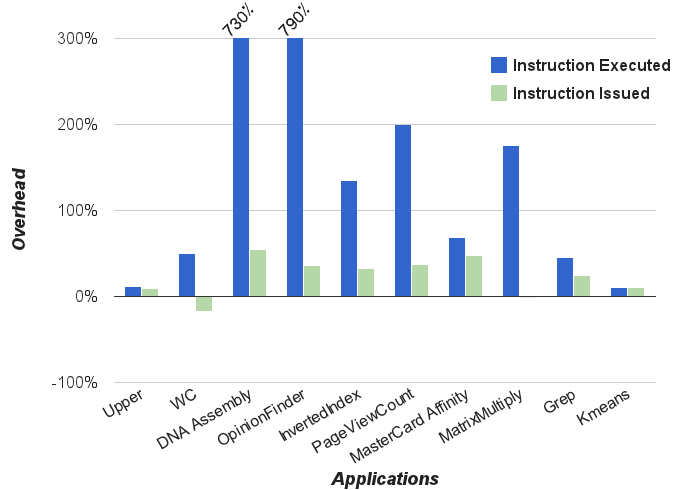
\includegraphics[scale=0.23]{4instructionIssueOverhead.png}
\caption{Instruction executed and issued overhead of S-L1.}
\label{fig:instexecissuedoverhead}
\end{figure}

S-L1 has significant overhead because it is implemented in software and extra instructions need to be executed for each memory access.
Figure~\ref{fig:instexecissuedoverhead} depicts the increase in the number of instructions, both executed and issued, under S-L1.
Executed instructions are the total number of instructions completed, while 
issued instructions also count the times an instruction is ``replayed'' because it
encountered a long latency event such as a memory load.

The increase in the number of executed instructions is significant: 220\% on average. 
The reason is obvious: each memory access instruction is transformed to additionally call a function that needs to be executed. 
On the other hand, the increase in the number of issued instructions is more reasonable:
only 25\% on average. 
(For \texttt{wc} and \texttt{MatrixMultiply} the number of issued instructions actually decreases.)
The reason issued instructions increase less than executed instructions is that S-L1 provides for improved memory performance, which reduces the number of required 
instruction replays.


\begin{figure}[t]
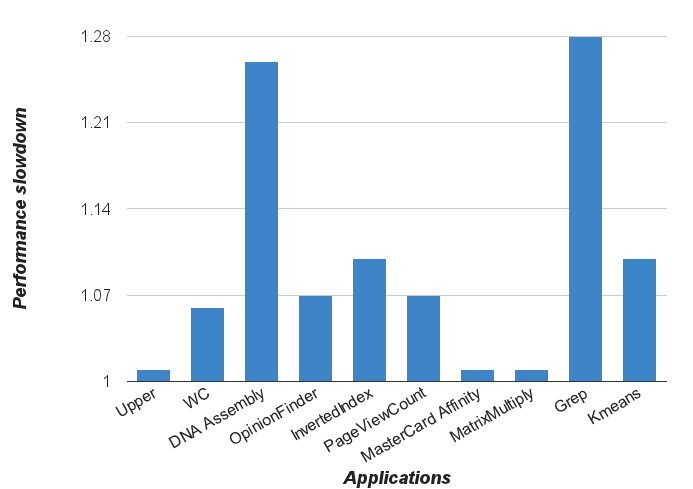
\includegraphics[scale=0.29]{7cachingOverhead.png}
\caption{Overhead of S-L1 when no cache line is assigned to threads.}
\label{fig:sl1overhead}
\end{figure}

To evaluate the overhead S-L1 introduces for data structures that are not cached, we ran our benchmarks with S-L1, but with all data structures marked as non-cacheable.
Figure~\ref{fig:sl1overhead} shows the overhead incurred in this case: 8\% on average.
Based on our experiments, the monitoring phase accounts for less than 1\% of this overhead. 
The rest of the overhead is attributed to executing the memory access function that is called for each memory access.
As suggested in Section~\ref{}, one potential way to avoid this overhead is have the compiler not
transform memory accesses to data structures that are found not worthy of caching -- e.g. a data
structure that is statically known not exhibit any caching benefit.


\subsection{Effect of S-L1 cache line size}


\begin{figure}[t]
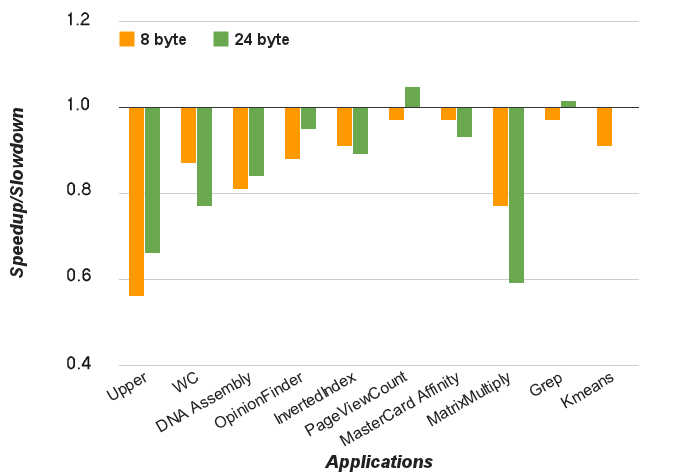
\includegraphics[scale=0.29]{6differentCachelineSizes.png}
\caption{Comparison of different cache line sizes.}
\label{fig:cachelinesize}
\end{figure}

Figure~\ref{fig:cachelinesize} compares the overall performance of applications when using different variations of S-L1 using different cache line sizes. 
Specifically, we show the performance improvement/loss for 8-byte and 24-byte cache lines over 16-byte cache lines.
In most cases, 16-byte cache lines seems to be best choice. 
As we described in Section~\ref{}, we believe this is mainly because 16-bytes is the widest available load/store size on GPU ISA and hence, the entire cache line can be read/written with one memory access.

Decreasing the cache line size to 8-bytes impacts performance negatively in every case, since the cache then typically needs to execute the inserted memory access function twice as often for a fixed amount of streaming data to be processed by the application. 
Note that our benchmarks primarily consist of streaming applications that have high spatial locality and that consume most of the data in a cache lines.

Increasing the cache line size to 24-bytes also reduces performance in all but two cases, mainly
because 24 bytes do not provide much additional benefit over 16 bytes, yet require two memory accesses to fill a cache line instead of one.

%\todo{Huh????} %this was not supposed to be included in the actual paper%
%As we described in Section~\ref{}, we believe that a wider load/store size in future GPUs (e.g.
%32-bytes) can be very helpful in increasing the bandwidth exhibited by applications and this caching
%layer.



